\begin{figure}[h!]
	\adjustbox{center}{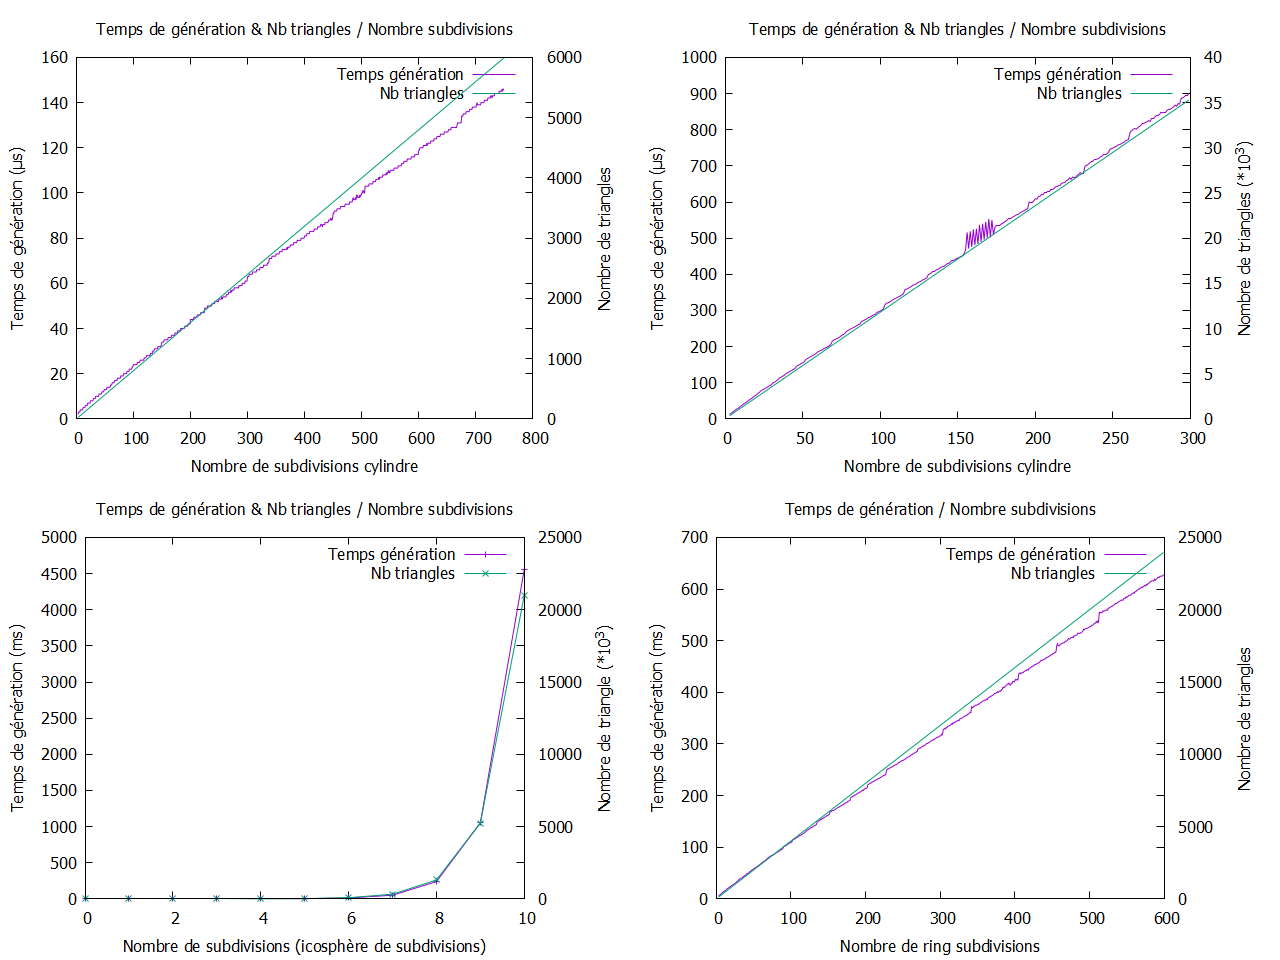
\includegraphics[width=1\textwidth]{Captures/allBenchmarksTriangles.png}}

	\caption{Temps de génération pour les maillages simples implémentés en fonction du nombre de subdivisions}
\end{figure}
\FloatBarrier

Toutes les primitives à l'exception de l'icopshère évoluent en temps linéaire quand leur nombre de subdivisions 
augmente et c'est le comportement auquel on pourrait s'attendre. L'icosphère évolue en $4^n$ avec $n$ le nombre 
de subdivisions. C'est également ce à quoi on s'attend puisque la subdivision dyadique multiplie par 4 le nombre 
de triangles à chaque subdivision.
